% Compile with: pdflatex lecture_32.tex
% Requires: amsmath, amssymb, amsthm, mathtools, xcolor, mdframed,
%           enumitem, hyperref, pagecolor, microtype, tikz

\documentclass[11pt]{article}
\usepackage[margin=1in]{geometry}
\usepackage{amsmath, amssymb, amsthm}
\usepackage{mathtools}
\usepackage{xcolor}
\usepackage{mdframed}
\usepackage{enumitem}
\usepackage{hyperref}
\usepackage{pagecolor}
\usepackage[expansion=false]{microtype}
\usepackage{tikz}
\usetikzlibrary{arrows.meta, positioning, shapes.geometric}

% ---------- Colour palette ----------
\definecolor{cream}{HTML}{FFFDF5}
\definecolor{defblue}{HTML}{1A4A7A}
\definecolor{thmgreen}{HTML}{1A5C3A}
\definecolor{warnAmber}{HTML}{7A4A00}
\definecolor{dangerRed}{HTML}{7A1A1A}
\definecolor{boxbluebg}{HTML}{EBF3FB}
\definecolor{boxgreenbg}{HTML}{EBF7EF}
\definecolor{boxamberbg}{HTML}{FDF5E6}
\definecolor{boxredbg}{HTML}{FBEBEB}
\pagecolor{cream}

% ---------- Theorem styles ----------
\newtheoremstyle{defstyle}    {8pt}{8pt}{\normalfont}{0pt}{\bfseries\color{defblue}} {.}{0.5em}{}
\newtheoremstyle{thmstyle}    {8pt}{8pt}{\normalfont}{0pt}{\bfseries\color{thmgreen}}{.}{0.5em}{}
\newtheoremstyle{notstyle}    {8pt}{8pt}{\normalfont}{0pt}{\bfseries\color{warnAmber}}{.}{0.5em}{}
\newtheoremstyle{cautionstyle}{8pt}{8pt}{\normalfont}{0pt}{\bfseries\color{dangerRed}}{.}{0.5em}{}

\theoremstyle{defstyle}
\newtheorem{definition}{Definition}[section]

\theoremstyle{thmstyle}
\newtheorem{theorem}{Theorem}[section]
\newtheorem{corollary}[theorem]{Corollary}

\theoremstyle{notstyle}
\newtheorem*{remark}{Remark}
\newtheorem*{example}{Example}

\theoremstyle{cautionstyle}
\newtheorem*{caution}{Caution}

% ---------- Boxes ----------
\newmdenv[
  backgroundcolor=boxbluebg, linecolor=defblue, linewidth=2pt,
  topline=false, rightline=false, bottomline=false,
  innerleftmargin=10pt, innerrightmargin=10pt,
  innertopmargin=6pt, innerbottommargin=6pt,
  skipabove=8pt, skipbelow=8pt
]{defbox}

\newmdenv[
  backgroundcolor=boxgreenbg, linecolor=thmgreen, linewidth=2pt,
  topline=false, rightline=false, bottomline=false,
  innerleftmargin=10pt, innerrightmargin=10pt,
  innertopmargin=6pt, innerbottommargin=6pt,
  skipabove=8pt, skipbelow=8pt
]{thmbox}

\newmdenv[
  backgroundcolor=boxamberbg, linecolor=warnAmber, linewidth=2pt,
  topline=false, rightline=false, bottomline=false,
  innerleftmargin=10pt, innerrightmargin=10pt,
  innertopmargin=6pt, innerbottommargin=6pt,
  skipabove=8pt, skipbelow=8pt
]{notebox}

\newmdenv[
  backgroundcolor=boxredbg, linecolor=dangerRed, linewidth=2pt,
  topline=false, rightline=false, bottomline=false,
  innerleftmargin=10pt, innerrightmargin=10pt,
  innertopmargin=6pt, innerbottommargin=6pt,
  skipabove=8pt, skipbelow=8pt
]{cautionbox}

% ---------- Macros ----------
\newcommand{\Z}{\mathbb{Z}}
\newcommand{\N}{\mathbb{N}}
\newcommand{\R}{\mathbb{R}}
\newcommand{\Np}{\mathbb{N}^{+}}
\newcommand{\Pow}{\mathcal{P}}

\begin{document}

\begin{center}
  {\Large\bfseries Lecture 32 --- Infinity}\\[4pt]
  {\normalsize CS 173: Discrete Structures \quad$\cdot$\quad Infinite sets, Dedekind infinity, Hilbert's hotel}\\[2pt]
  {\small\color{gray} University of Illinois at Urbana-Champaign}
\end{center}
\vspace{1em}\hrule\vspace{1.5em}

% ============================================================
\section{Recall: \texorpdfstring{$\binom{n}{k}$}{n choose k}}
% ============================================================

From Chapter 6 of the reference, for a set $X$ with $|X| = n$ and $n, k \in \N$,
\[
  \binom{n}{k} \;:=\; \bigl|\{\, Z \in \Pow(X) \;\bigl|\; |Z| = k \,\}\bigr|.
\]
That is, $\binom{n}{k}$ --- read \emph{``$n$ choose $k$''} --- is the number of subsets of cardinality $k$ taken from a set of cardinality $n$.

\begin{notebox}
\begin{example}
Let $n = 5$, $k = 2$, and take $X = \{a, b, c, d, e\}$, so $|X| = 5$. One particular subset of cardinality $2$ is $Z = \{b, c\}$. Counting all such two-element subsets gives
\[
  \binom{5}{2} = 10.
\]
\end{example}
\end{notebox}

% ============================================================
\section{What does ``infinite'' mean?}
% ============================================================

So far we have only counted finite sets. To do cardinality \emph{at scale}, we need a precise notion of an infinite set.

\begin{defbox}
\begin{definition}[Infinite set]
A set $X$ is \textbf{infinite} iff
\[
  (\forall n \in \N)\bigl(\, |X| \neq |[n]| \,\bigr),
\]
where $[n] = \{1, 2, \ldots, n\}$ is the standard finite set of size $n$. In words: $X$ is infinite iff its cardinality matches no finite cardinality.
\end{definition}
\end{defbox}

\begin{notebox}
\begin{remark}
This is the ``negative'' definition of infinity --- $X$ is infinite precisely when no bijection $X \to [n]$ exists, for any $n \in \N$. Soon we'll see a striking ``positive'' characterization (Dedekind's), where infiniteness is detected by a strange internal symmetry.
\end{remark}
\end{notebox}

% ============================================================
\section{Dedekind infinite vs.\ Dedekind finite}
% ============================================================

A finite set has the property that no proper subset can match its size --- if you remove anything, it gets strictly smaller. Dedekind's idea is to flip this: an infinite set is one that \emph{can} have a proper subset of the same size.

\begin{defbox}
\begin{definition}[Dedekind infinite]
A set $X$ is \textbf{Dedekind infinite} iff
\[
  (\exists Y)\bigl(\, Y \subseteq X \;\land\; Y \neq X \;\land\; |X| = |Y| \,\bigr).
\]
That is, $X$ has a proper subset $Y$ with the same cardinality as $X$ itself.
\end{definition}
\end{defbox}

\begin{defbox}
\begin{definition}[Dedekind finite]
Given a set $X$, we say $X$ is \textbf{Dedekind finite} iff
\[
  (\forall Y)\bigl(\, Y \subseteq X \;\land\; Y \neq X \;\Rightarrow\; |Y| < |X| \,\bigr).
\]
Every proper subset is \emph{strictly} smaller.
\end{definition}
\end{defbox}

\begin{notebox}
\begin{remark}[Finite sets behave nicely]
For finite sets $A, B$:
\[
  A \subseteq B \;\land\; A \neq B \;\Longrightarrow\; |A| < |B| \;\;\text{and hence}\;\; |A| \neq |B|.
\]
So every finite set is Dedekind finite --- this is the intuition the definition is trying to capture.
\end{remark}
\end{notebox}

\begin{cautionbox}
\begin{caution}
The strict inequality $|A| < |B|$ is the right tool only when $A \subseteq B$ and $A \neq B$. Without proper containment, $|A| < |B|$ alone tells you nothing about subset structure (e.g.\ $\{1,2\}$ and $\{3,4,5\}$).
\end{caution}
\end{cautionbox}

% ============================================================
\section{Infinite \texorpdfstring{$\iff$}{iff} Dedekind infinite}
% ============================================================

The two definitions of ``infinite'' --- the negative one (no finite cardinality) and the positive one (a proper subset of the same size) --- coincide.

\begin{thmbox}
\begin{theorem}[Equivalence of infinity]
A set $X$ is infinite if and only if $X$ is Dedekind infinite.
\end{theorem}
\end{thmbox}

\begin{notebox}
\begin{remark}
We won't prove the full equivalence today --- the $(\Leftarrow)$ direction is straightforward, while $(\Rightarrow)$ requires the Axiom of Choice in the general case. The next two theorems are concrete instances of the Dedekind side: each exhibits an infinite set together with a proper subset of equal size.
\end{remark}
\end{notebox}

% ============================================================
\section{First example: \texorpdfstring{$|\Np| = |\N|$}{|N+|=|N|}}
% ============================================================

Recall $\N = \{0, 1, 2, \ldots\}$ and $\Np = \{1, 2, 3, \ldots\}$. So $\Np \subseteq \N$ and $\Np \neq \N$ (since $0 \in \N \setminus \Np$). Despite this, the two have the same cardinality.

\begin{thmbox}
\begin{theorem}
$|\Np| = |\N|$.
\end{theorem}
\end{thmbox}

\begin{proof}
Recall $|\Np| = |\N| \iff \exists f$ with $f : \N \to \Np$ a bijection. Consider $f : \N \to \Np$ given by, for any $n \in \N$,
\[
  f(n) := n + 1.
\]
\textbf{Injective.} Suppose $f(m) = f(n)$, i.e.\ $m + 1 = n + 1$. Then $m = n$.

\textbf{Surjective.} Let $y \in \Np$, so $y \geq 1$. Then $y - 1 \in \N$ and $f(y - 1) = (y - 1) + 1 = y$.

Hence $f$ is a bijection, so $|\Np| = |\N|$.
\end{proof}

\begin{notebox}
\begin{remark}
This already shows $\N$ is Dedekind infinite: $\Np$ is a proper subset of $\N$ with $|\Np| = |\N|$. Witnessing the equivalence theorem in the simplest possible setting.
\end{remark}
\end{notebox}

% --- TikZ diagram for f(n) = n+1 ---
\begin{center}
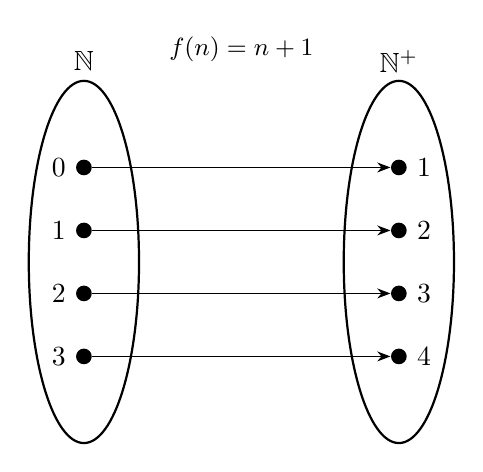
\begin{tikzpicture}[>=Stealth,
    dot/.style={circle, fill, inner sep=2pt}]

  % left oval (N)
  \draw[thick] (0, 1) ellipse (0.7cm and 2.3cm);
  \node at (0, 3.55) {$\N$};

  % right oval (N+)
  \draw[thick] (4, 1) ellipse (0.7cm and 2.3cm);
  \node at (4, 3.55) {$\Np$};

  % dots on left at y = 2.2, 1.4, 0.6, -0.2
  \node[dot, label=left:{$0$}]  (a0) at (0,  2.2) {};
  \node[dot, label=left:{$1$}]  (a1) at (0,  1.4) {};
  \node[dot, label=left:{$2$}]  (a2) at (0,  0.6) {};
  \node[dot, label=left:{$3$}]  (a3) at (0, -0.2) {};

  % dots on right
  \node[dot, label=right:{$1$}] (b1) at (4,  2.2) {};
  \node[dot, label=right:{$2$}] (b2) at (4,  1.4) {};
  \node[dot, label=right:{$3$}] (b3) at (4,  0.6) {};
  \node[dot, label=right:{$4$}] (b4) at (4, -0.2) {};

  \draw[->] (a0) -- (b1);
  \draw[->] (a1) -- (b2);
  \draw[->] (a2) -- (b3);
  \draw[->] (a3) -- (b4);

  \node[font=\bfseries\small] at (2, 3.7) {$f(n) = n+1$};
\end{tikzpicture}
\end{center}

% ============================================================
\section{Second example: \texorpdfstring{$|\Z| = |\N|$}{|Z|=|N|}}
% ============================================================

The integers stretch in two directions; $\N$ in only one. Yet they have the same size.

\begin{thmbox}
\begin{theorem}
$|\Z| = |\N|$.
\end{theorem}
\end{thmbox}

\begin{proof}
Consider $f : \Z \to \N$ defined by
\[
  f(x) := \begin{cases} 2x & \text{if } x \geq 0, \\ -2x - 1 & \text{if } x < 0, \end{cases}
\]
and $g : \N \to \Z$ defined by $g(x) := x$.

The map $f$ sends non-negative integers to even naturals ($0 \mapsto 0$, $1 \mapsto 2$, $2 \mapsto 4$, $\ldots$) and negative integers to odd naturals ($-1 \mapsto 1$, $-2 \mapsto 3$, $-3 \mapsto 5$, $\ldots$). One can check $f$ is a bijection: every natural number is reached exactly once, even numbers from the non-negative branch and odd numbers from the negative branch.

Hence $|\Z| = |\N|$.
\end{proof}

\begin{notebox}
\begin{remark}
The map $g : \N \to \Z$ given by $g(x) = x$ is the obvious inclusion --- it shows $\N \subseteq \Z$, hence $|\N| \leq |\Z|$. Combined with the bijection $f$, we get equality. Listing $\Z$ as
\[
  0, \; -1, \; 1, \; -2, \; 2, \; -3, \; 3, \; \ldots
\]
gives the same bijection in disguise --- $f^{-1}$ reads off the $n$-th term of this list.
\end{remark}
\end{notebox}

% --- Bijection picture for Z <-> N ---
\begin{center}
\renewcommand{\arraystretch}{1.5}
\begin{tabular}{|c|c|c|c|c|c|c|c|}
\hline
$x \in \Z$ & $0$ & $-1$ & $1$ & $-2$ & $2$ & $-3$ & $3$ \\
\hline
$f(x) \in \N$ & $0$ & $1$ & $2$ & $3$ & $4$ & $5$ & $6$ \\
\hline
\end{tabular}
\end{center}

% ============================================================
\section{Hilbert's hotel}
% ============================================================

The two theorems above are not isolated tricks --- they are the discrete shadow of a single picture due to David Hilbert. The Grand Hotel is a thought experiment in which the strangeness of infinite cardinality becomes operational: rooms can be ``made'' for new guests in a fully booked hotel, simply by relabelling.

\begin{notebox}
\begin{remark}[Setup]
Imagine a hotel with rooms labelled by $\Np = \{1, 2, 3, \ldots\}$ --- one room for every positive integer. Suppose every room is occupied: for each $n \in \Np$, room $n$ houses guest $G_n$.
\end{remark}
\end{notebox}

\subsection*{Scenario 1: One new guest arrives}

A traveller shows up at the front desk. With finitely many rooms, the manager would say ``sorry, full.'' In the Grand Hotel, instead:

\begin{quote}
\emph{Every guest $G_n$ moves from room $n$ to room $n + 1$.}
\end{quote}

After the shift, room $1$ is empty. The new guest takes room $1$. No one is left out, because the map $n \mapsto n + 1$ is a bijection $\Np \to \Np \setminus \{1\}$ --- exactly the bijection underlying $|\Np| = |\N|$ from \S5.

\begin{thmbox}
\begin{theorem}[One new guest]
There is a bijection $\Np \to \Np$ that ``frees up'' room $1$, namely $n \mapsto n + 1$ as a map onto $\{2, 3, 4, \ldots\}$.
\end{theorem}
\end{thmbox}

\subsection*{Scenario 2: Countably many new guests arrive}

Now a bus pulls up carrying guests $H_1, H_2, H_3, \ldots$ --- one for each positive integer.

\begin{quote}
\emph{Every guest $G_n$ moves from room $n$ to room $2n$.}
\end{quote}

After the shift, the even rooms $\{2, 4, 6, \ldots\}$ are occupied by old guests, and the odd rooms $\{1, 3, 5, \ldots\}$ are empty. Place new guest $H_k$ in room $2k - 1$.

\begin{notebox}
\begin{remark}
Old guests use the bijection $\Np \to 2\Np$ ($n \mapsto 2n$); new guests use the bijection $\Np \to 2\Np - 1$ ($k \mapsto 2k - 1$). Together they exhibit a bijection
\[
  \Np \sqcup \Np \;\longrightarrow\; \Np,
\]
which is precisely the content of $|\Z| = |\N|$ from \S6 in another guise (negative integers $\sim$ new guests, non-negative integers $\sim$ old guests).
\end{remark}
\end{notebox}

\begin{center}
\renewcommand{\arraystretch}{1.5}
\begin{tabular}{|l|l|l|}
\hline
\textbf{Scenario} & \textbf{Reassignment} & \textbf{Underlying bijection} \\
\hline
$1$ new guest & $G_n \to$ room $n+1$ & $n \mapsto n+1$ \\
Bus of $\Np$ guests & $G_n \to$ room $2n$, \ $H_k \to$ room $2k-1$ & $\Np \sqcup \Np \to \Np$ \\
\hline
\end{tabular}
\end{center}

\begin{cautionbox}
\begin{caution}
The hotel argument relies on \emph{simultaneous} relabelling. You cannot move the guests one at a time and expect to reach a stable configuration --- there is no ``last'' guest to move. The bijection is a single global act, not a process.
\end{caution}
\end{cautionbox}

\begin{notebox}
\begin{remark}[Why this matters]
Hilbert's hotel is the first hint that ``infinite $+ 1 =$ infinite'' and ``infinite $+$ infinite $=$ infinite'' --- not as sloppy slogans but as honest cardinal equalities $|\N| + 1 = |\N|$ and $|\N| + |\N| = |\N|$. The Dedekind definition (\S3) makes this exact: a set is infinite precisely when it admits such a self-rearrangement.
\end{remark}
\end{notebox}

% ============================================================
\section{Summary}
% ============================================================

\begin{enumerate}[leftmargin=*]
  \item $\binom{n}{k}$ counts the $k$-subsets of an $n$-set: $\binom{n}{k} = |\{Z \in \Pow(X) : |Z| = k\}|$ when $|X| = n$.
  \item $X$ is \textbf{infinite} iff $|X|$ is not equal to $|[n]|$ for any $n \in \N$.
  \item $X$ is \textbf{Dedekind infinite} iff some proper subset $Y \subsetneq X$ satisfies $|Y| = |X|$; \textbf{Dedekind finite} iff every proper subset is strictly smaller.
  \item For finite $A, B$: $A \subsetneq B \Rightarrow |A| < |B|$ and $|A| \neq |B|$. Finite sets are Dedekind finite.
  \item $\text{infinite} \iff \text{Dedekind infinite}$ (stated; full proof deferred).
  \item $|\Np| = |\N|$ via $f(n) = n + 1$.
  \item $|\Z| = |\N|$ via $f(x) = 2x$ for $x \geq 0$, $f(x) = -2x - 1$ for $x < 0$.
  \item Hilbert's hotel concretizes both bijections: shift by one to make room for a guest, double up to make room for a bus.
\end{enumerate}

\begin{notebox}
\begin{remark}[Looking ahead]
We have only met one ``size of infinity'' so far --- the cardinality of $\N$, called \emph{countable}. The next natural question is whether \emph{every} infinite set has this size. Cantor's diagonal argument will show that $|\R| > |\N|$, exposing a strict hierarchy of infinities.
\end{remark}
\end{notebox}

\end{document}